\chapter{Prototype 1}

\section{activPal}
%Synes vi burde vise et eksempel av csv fila, og kanskje bare forklare veldig kort, men siden det egentlig ikke er oppgaven føler jeg at det hører til i appendix.
As mentioned in Section~\ref{sensorActivPal} the activPal classifies the accelerometer data into 3 different types of behaviour, this data can then be viewed through activPals proprietary software. There is an alternative to export the data in a \gls{csv} format, and there are several options as how the data should be presented or aggregated. It is possible to display raw accelerometer data or provide event based data where a new entry is created if the state has changed. A new line will then be written with the time, duration and state type every time the state changes. A more detailed overview of the \gls{csv} file can be found in (REF TO APENDIX)

For the purpose of our thesis the even based data \gls{csv} was the most suited basis for the type of information we would need for our visualizations.



\section{Paper sketches}
All the sketches described in this section were created through a set of informal brainstorming sessions between the authors where we occasionally received input from other sources. This was an iterative process that spanned over five sessions. The sketches represent our first ideas on visualizations that would fulfil the initial requirements efficiently, while providing alternatives to choose from. 

%Were we not supposed to change the name of this subsection. We were, but nobody has a fucking clue of what it should be callled
\subsection{Fractional charts}
These type of charts show the sum of time spent sedentary, standing, and walking. Summing over the three classifications makes it easy to get an overview of the day as a whole. The drawback are that details are lost and it is not possible to pinpoint when each activity occurred during the day. Fractional charts were created to cover IR2 and are intended to give a general overview of the daily activity before spending time looking at more detailed visualizations. Additionally it can serve as an alert for patients with low activity levels, where majority of the chart would be filled with inactivity.

\subsubsection{Pie chart}
The pie chart is a standard way of showing the amount of time spent in each activity state. Due to the familiarity of the pie chart it will be easy to understand for both users and patients. A legend shows which colour represents each type of activity. The exact percentage for each activity state is also displayed.

\subsubsection{Symbolic}
A more symbolic approach is to remove the legend and instead use illustrations to convey which colour corresponds to which activity. To get more space for the illustrations the diagram uses boxes instead of pie slices to represent the distribution of each activity level. Though the box chart is not as much used as the pie chart, humans can intuitively compare sizes of different types of shapes as long as they are paces in close proximity. 

%Dette burde kanskje flyttes til running prototype? Sammen med andre ting vi fant ut ikke funket like bra i praksis som papir.
% REVIEW: Dessuten passer det ikke med det over.
% REVIEW: I don't think we should have this section at all, the changes to the visualizations that should be talked about are those that were done because of feedback form the focus groups.
%The first idea was to only use the illustrations~\ref{fig:symbolicPie}, without the boxes, and scale the height to represent the ratio between each activity classification. However this idea was discarded because it became apparent that it was too hard to identify the ratio between the different illustrations. This is much easier with boxes.

%We may have to redraw this picture compared to the explanation in this section?
% REVIEW: Yes that probably is a good idea.
%RESPONSE: I am unsure if we need to redraw, i think it's nice to have it there, shows that things have changed a bit. Rather changed descriptive text to "first idea"
\begin{figure}[h!]
	\centering
		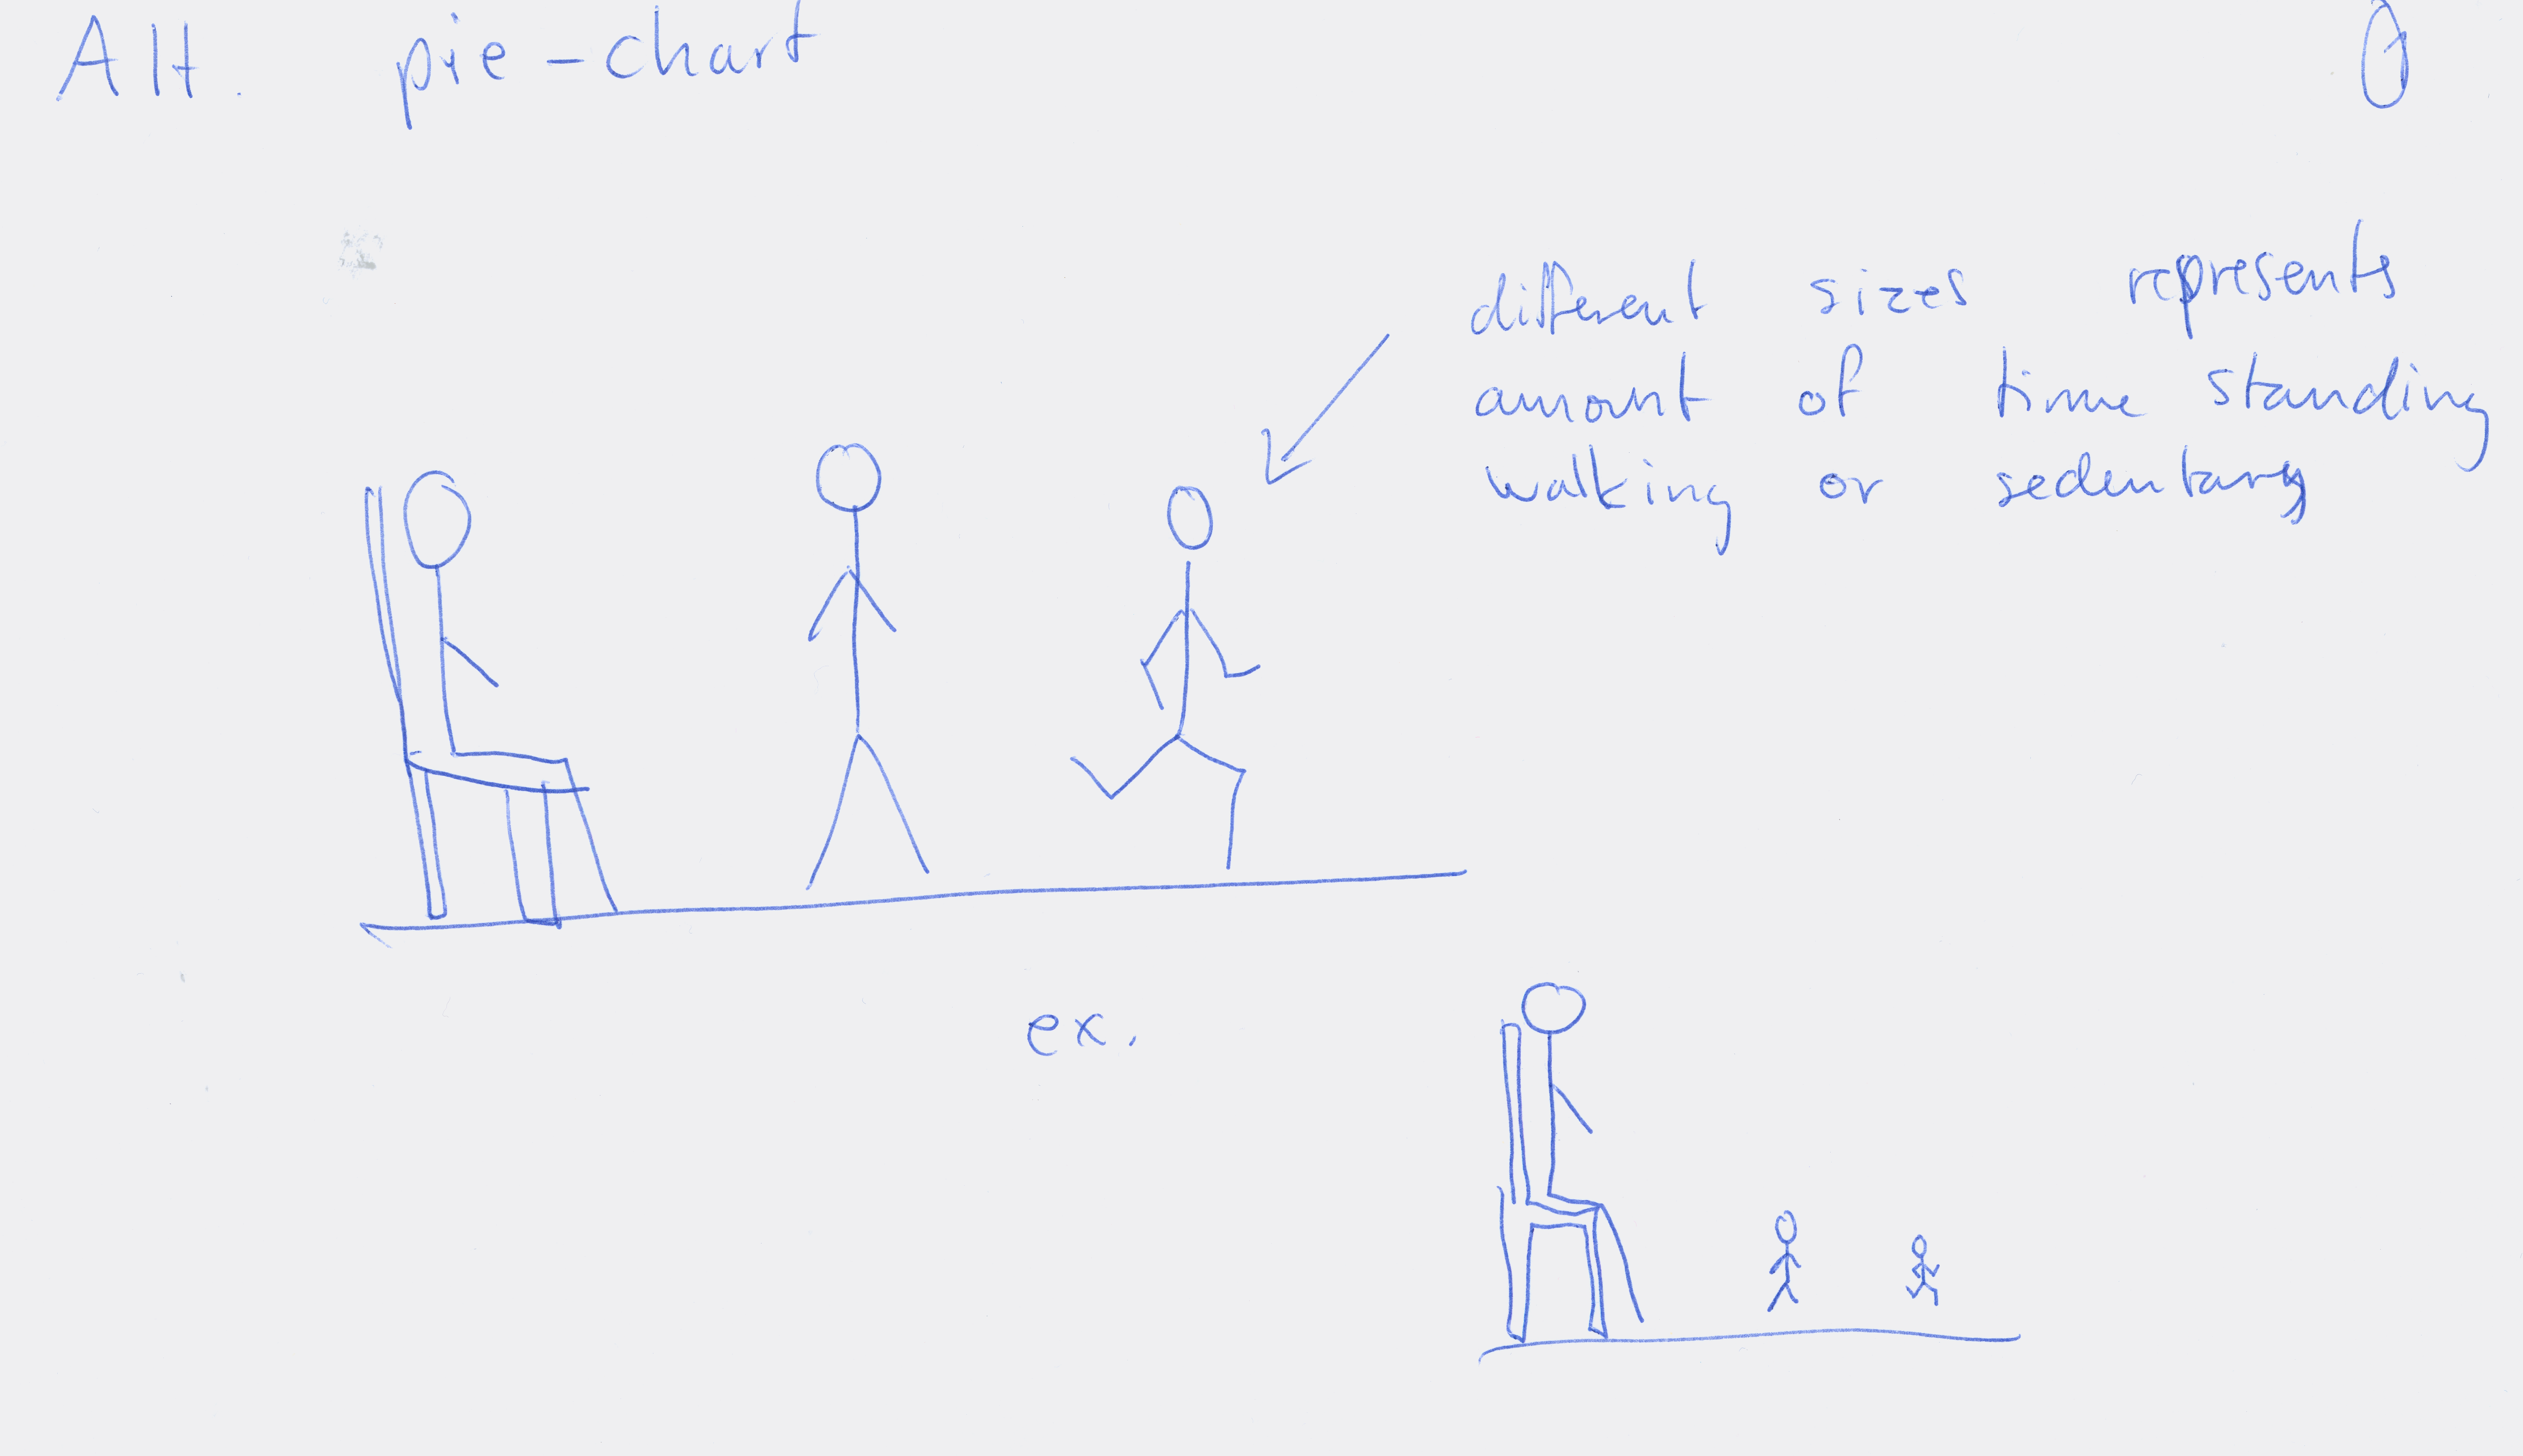
\includegraphics[width=0.7\textwidth]{stickSketch.png}
		\caption{\footnotesize Our first idea for a symbolic "pie chart"}
		\label{fig:symbolicPie}
\end{figure}

\subsubsection{Ball chart}
An alternative is to include more detail into a pie chart style, by using balls instead of normal pie slices. The balls are colour coded so that each colour reflects an activity state, while the size of the ball represent the continuous amount of time spent in the corresponding state. Each ball represents an interval of one of the classifications, so that many balls of one colour both represents the amount of that behaviour and shows how long each period of that behaviour was. Figure~\ref{fig:ballChart} shows an example of such a graph. The benefit with this type of graph is that one can easily identify long periods of sedentary behaviour. Taking small breaks with movement can help ``split up'' those balls, which is beneficial for ones health. By adding interactivity to the chart the user can select each ball and see what time it corresponds to. Overall the chart allows for the large balls to be easily spotted and the time of day quickly identified.

\begin{figure}[h!]
	\centering
		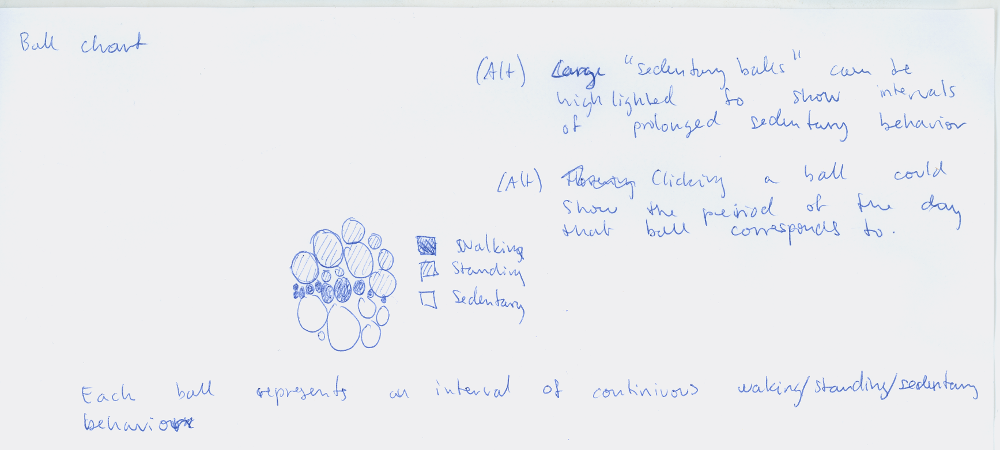
\includegraphics[width=0.7\textwidth]{ballChart.png}
		\caption{\footnotesize Rough drafts of the Ball chart}
		\label{fig:ballChart}
\end{figure}

\subsection{Timeline}
Timeline visualisations are effective at illustrating when various activities occurred during the day. The illustration uses a long horizontal bar that has different colours for different behavioural classification. These visualizations primarily address requirement IR3, IR5, and IR6. Such a bar can be used to identify points during the day where the subject is in a sedentary position for too long. By looking at multiple days, the user can detect patterns in the day where he needs to be more active.

\subsubsection{Continuous}
One approach to this visualization type is to create a continuous timeline that contains every little detail of activity. The continuous timeline is useful for quickly identifying periods of the day with unsatisfactory behaviour, but the detail can also be distracting and make it harder to read the graph.

\subsubsection{Blocks}
Instead of having a continuous scale, a blocked approach can be used, as seen in figure \ref{fig:timelineBlocks}. The timeline would be divided into 24 blocks, each block corresponding to an hour of the day. A gradient colour scale is used to represent the amount of activity inside the hour block. This makes it easy to identify hours of the day where the patient is inactive. 

\begin{figure}[h!]
	\centering
		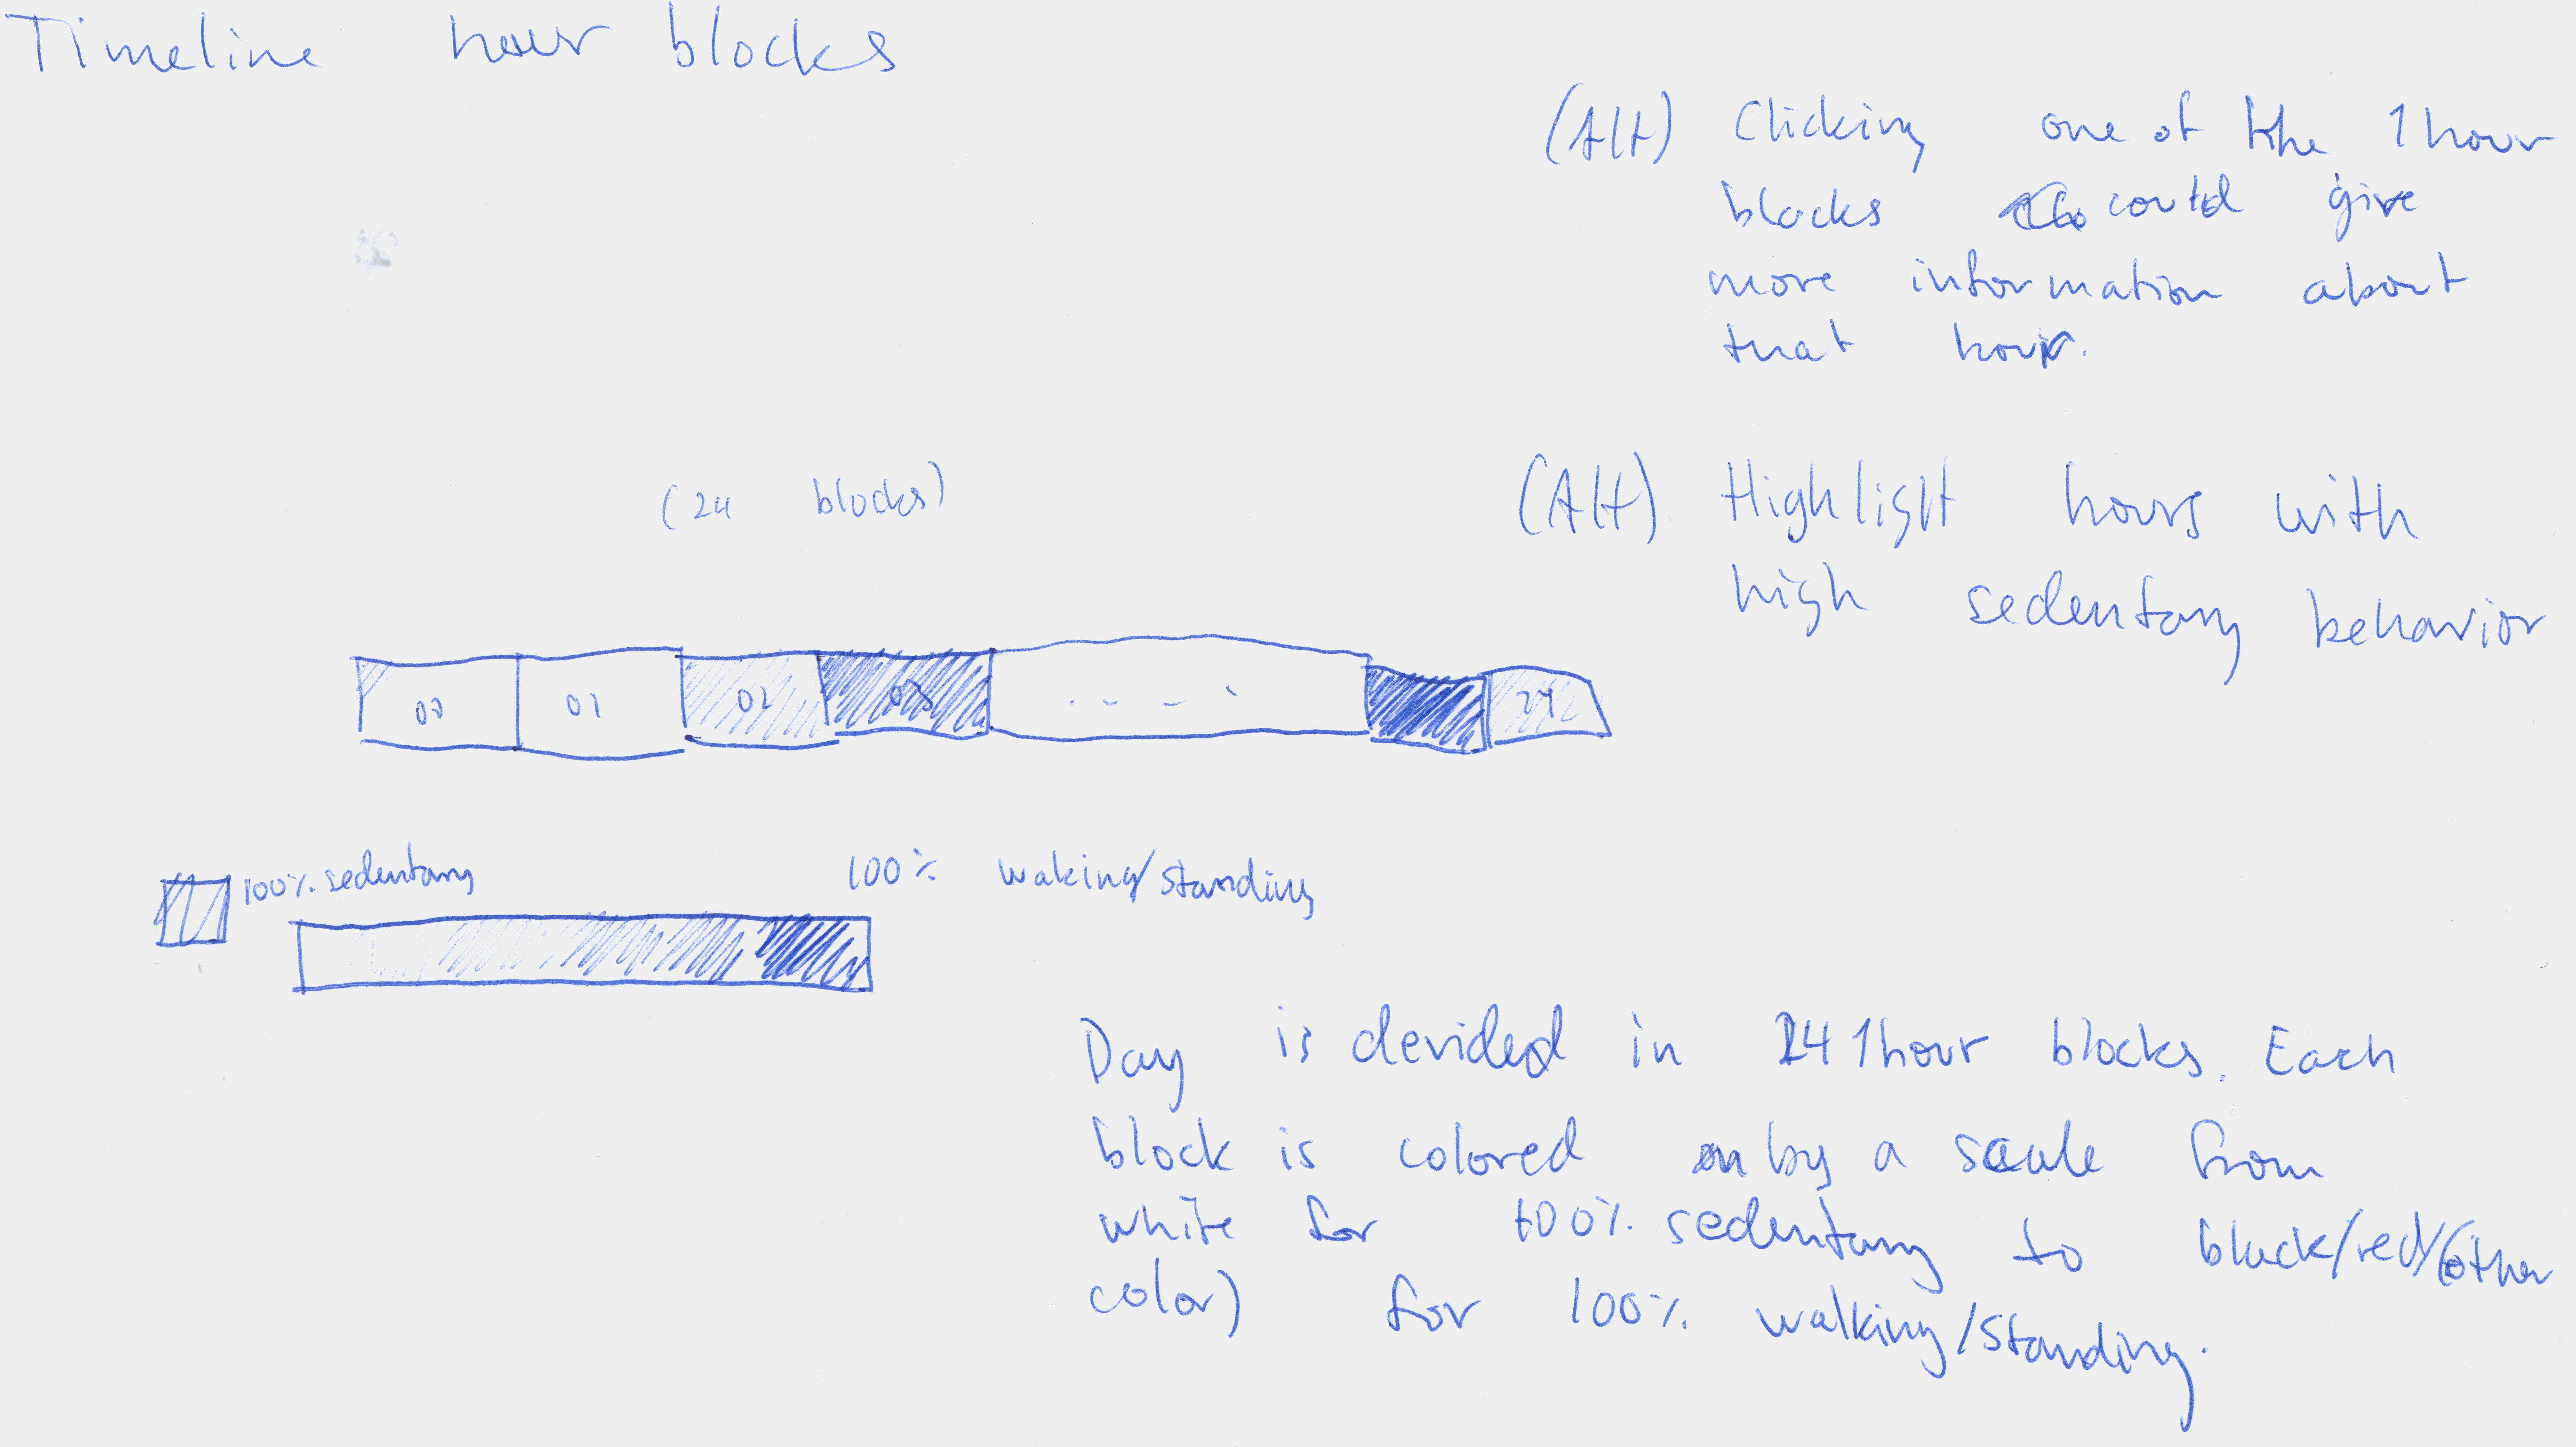
\includegraphics[width=0.7\textwidth]{timelineBlocksSketch.png}
		\caption{\footnotesize Timeline with hour blocks}
		\label{fig:timelineBlocks}
\end{figure}

\subsubsection{Clock}
A timeline may need some explanation before the user understands it properly. By creating two clocks instead of a long horizontal bar the user can more intuitively understand what the visualization is presenting. Since a clock has only 12 hours, two clocks are created to represent the entire day. To make it easier to identify day and night, a descriptive background is necessary, see figure \ref{fig:clock12}.

\begin{figure}[h!]
	\centering
		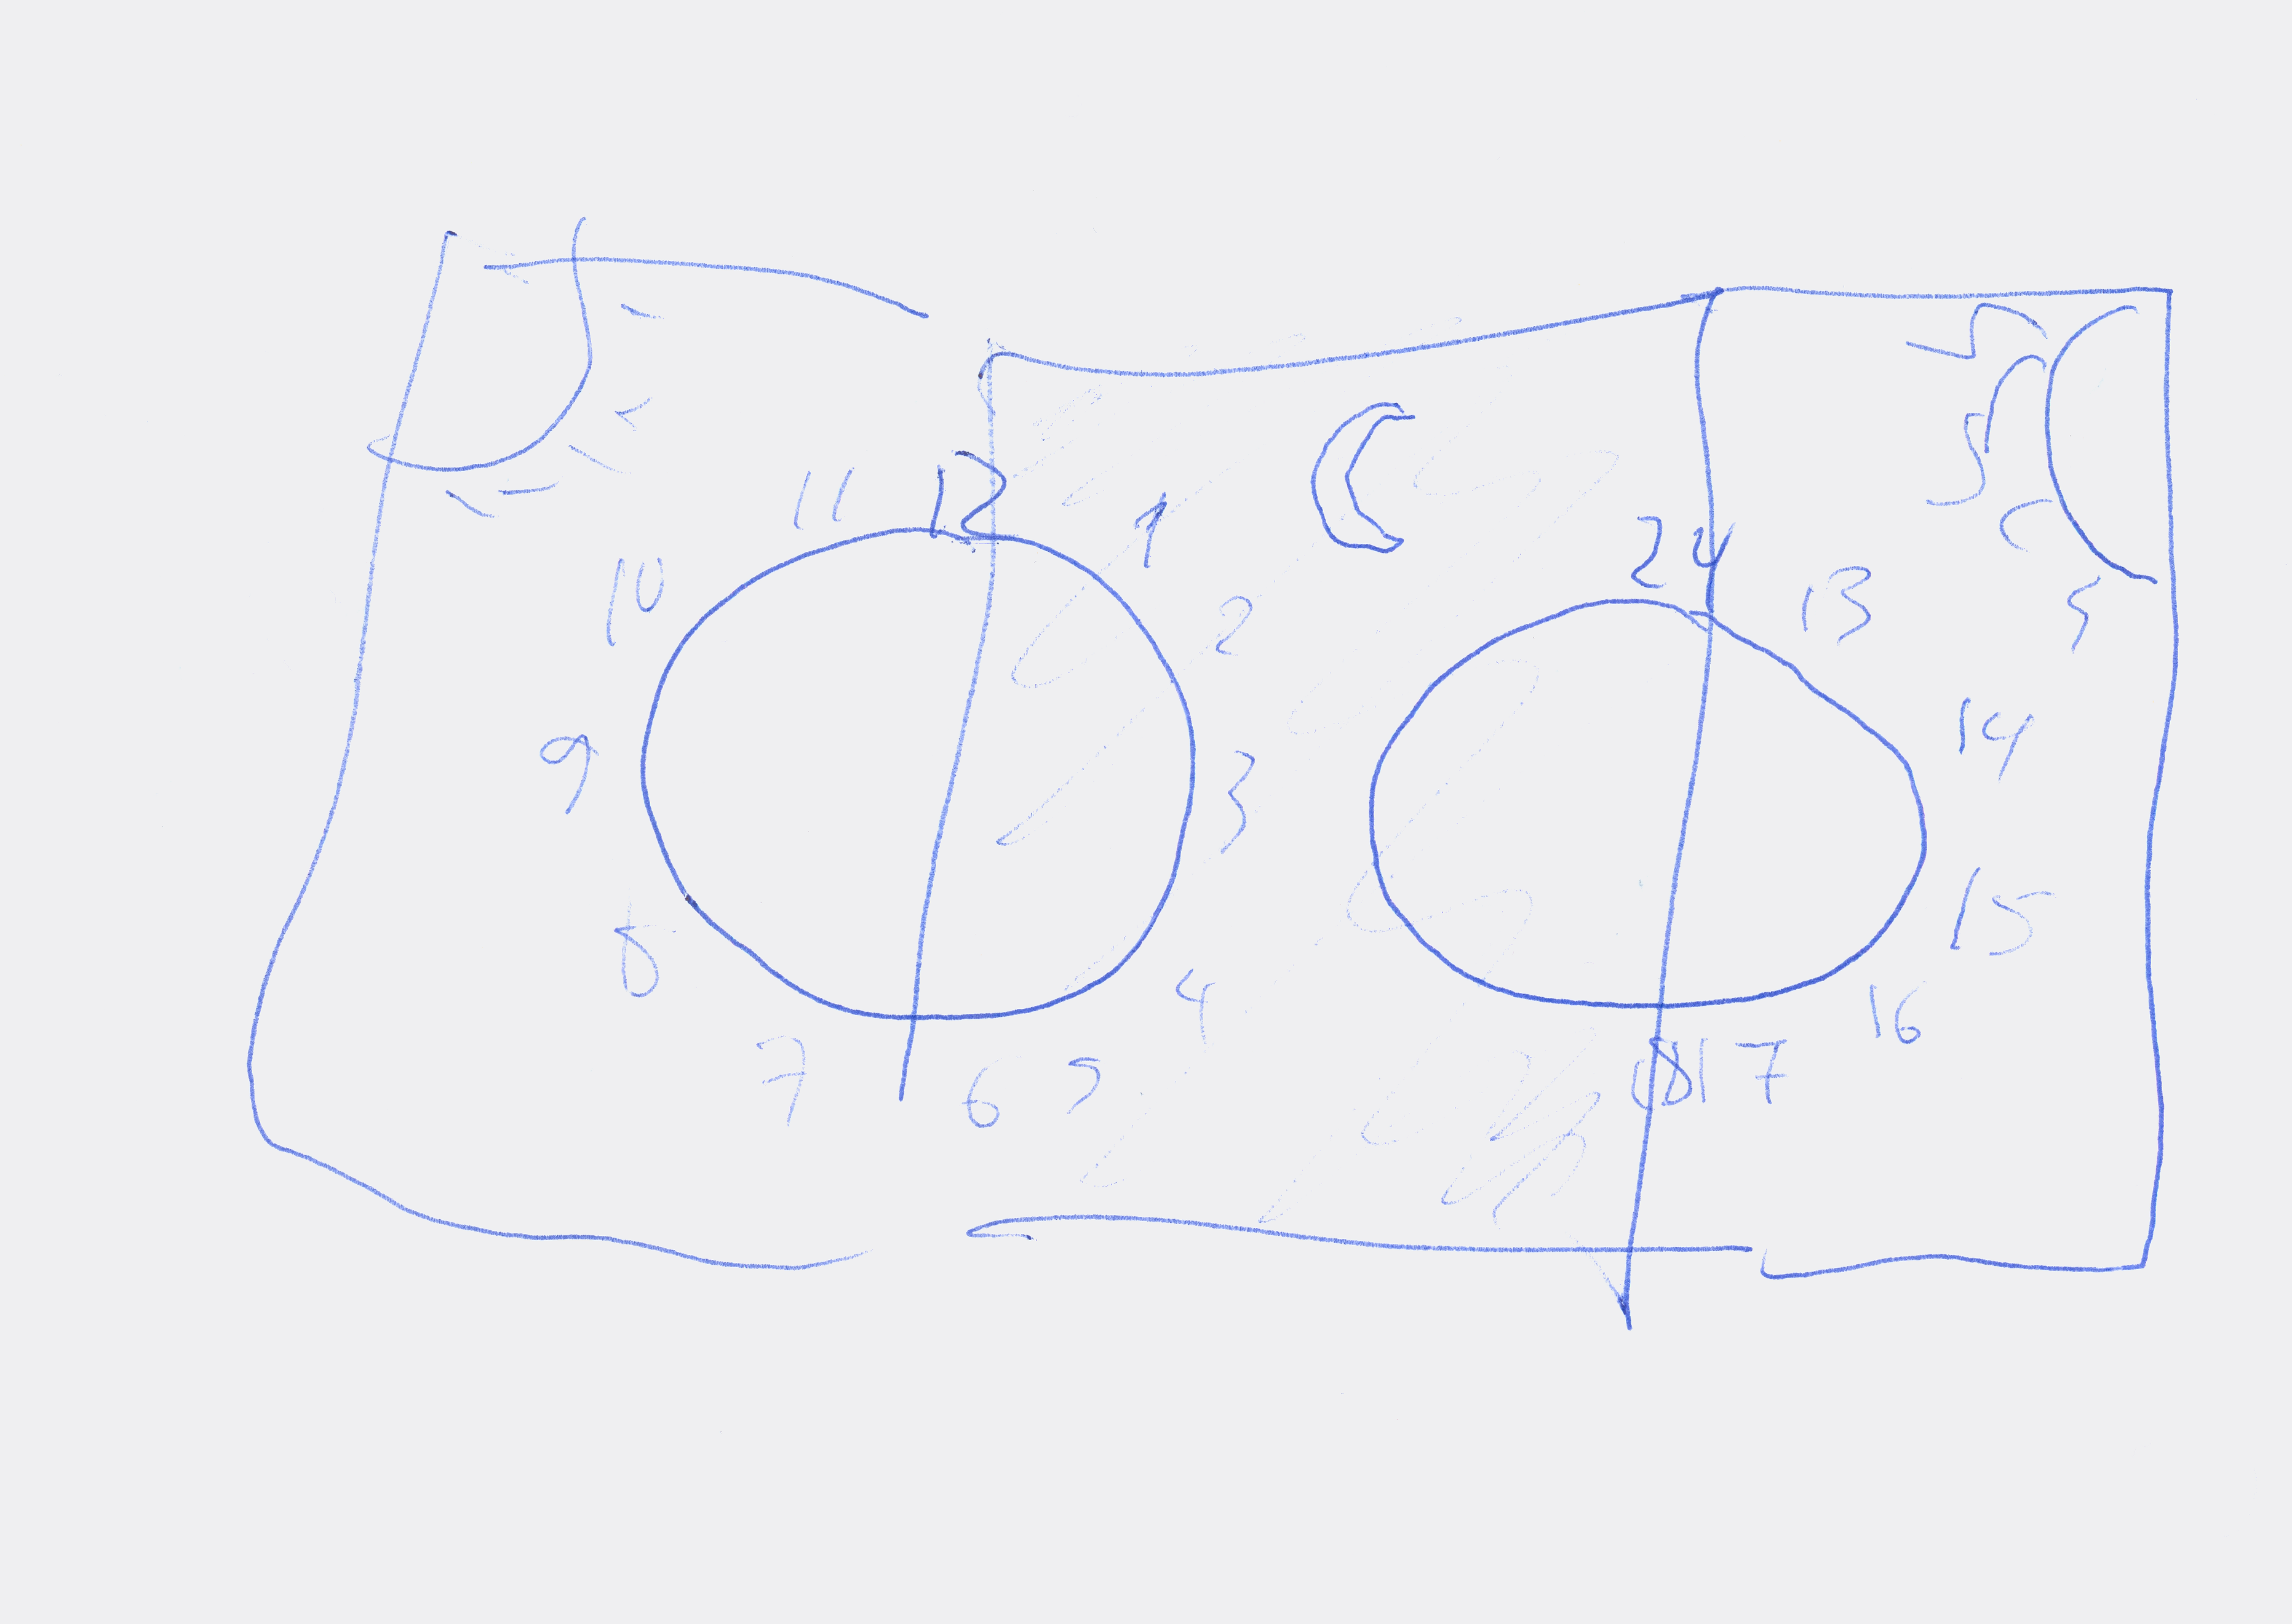
\includegraphics[width=0.7\textwidth]{clock12Sketch.png}
		\caption{\footnotesize Two 12 hour clocks show the activity of the day.}
		\label{fig:clock12}
\end{figure}

Another approach is to use one 24 hour clock. This makes it easier to see the transition between AM and PM, but 24 hour clocks are not natural, so it might be problematic for the user to understand.

\subsection{Week overview}
Getting an overview of the week as a whole can be useful as an introduction. By looking at an overview the user can quickly identify bad days that can then be investigated further. In other words they cover requirement IR1 and IR4. These visualizations could also be used as the top level of an interactive application. Each day could then be clicked to show either a timeline or pie chart.

\subsubsection{Day classification}
By calculating the overall activity level and classifying the days into three categories the user can easily see which days he need to be more active and which days the activity level is satisfactory. In our sketch, see figure \ref{fig:smileyWeek} the three different classifications are illustrated by smilies (smiling face for active days, and sad face for inactive days).

\begin{figure}[h!]
	\centering
		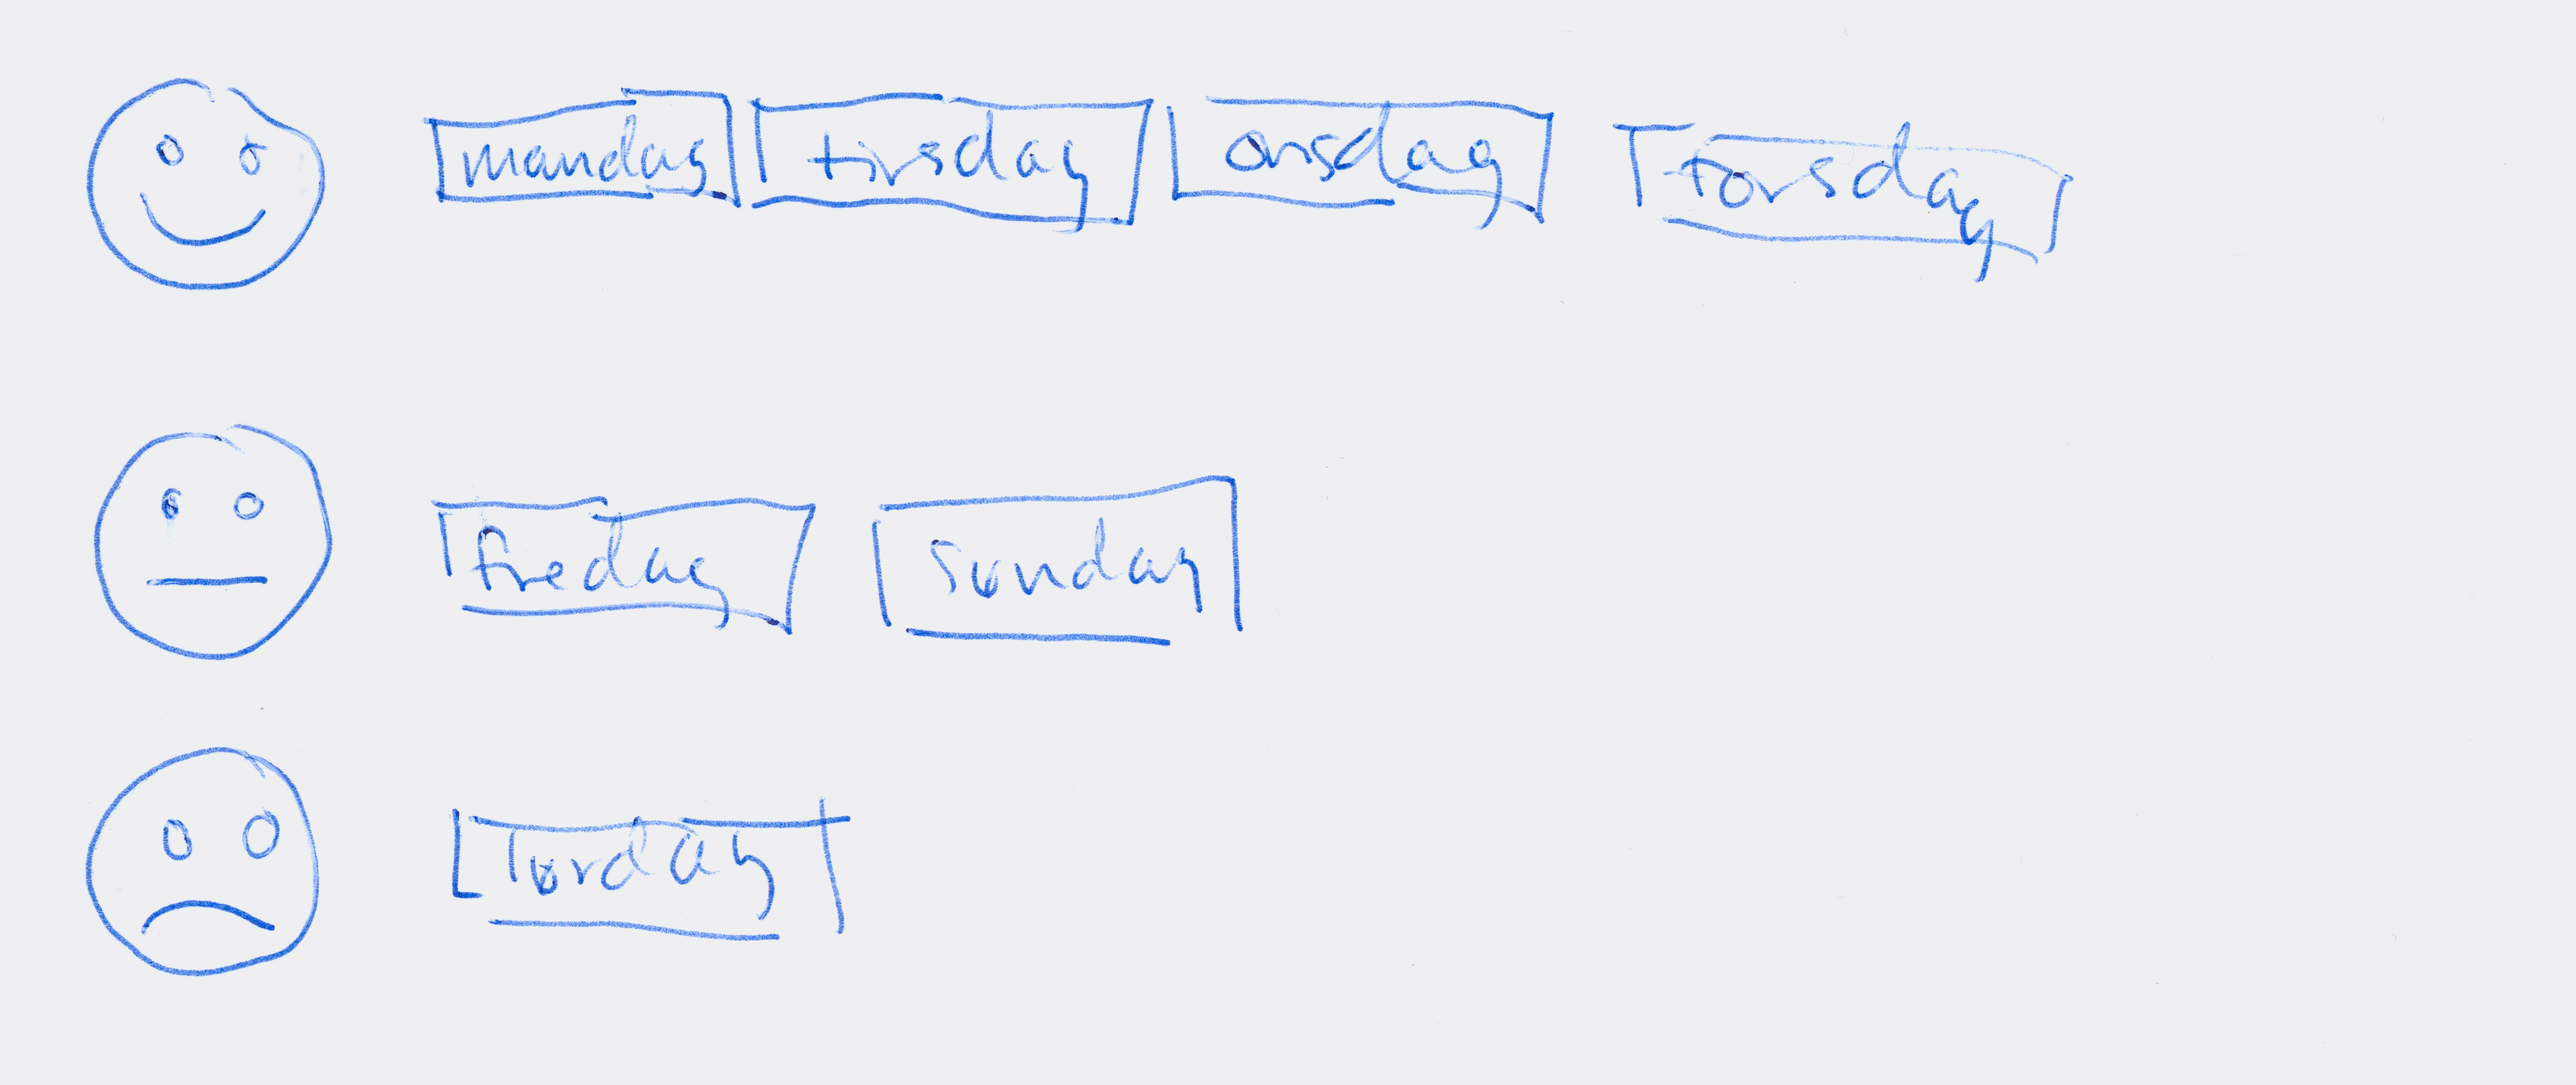
\includegraphics[width=0.7\textwidth]{smileyWeekSketch.png}
		\caption{\footnotesize Week overview with each day classified into one of three categories.}
		\label{fig:smileyWeek}
\end{figure}

A more complex version of the above chart, see figure \ref{fig:detailedWeek} is to show a square for each day, while still using the same classification into sad and happy smilies. Each day square will then contain 24 smaller squares that represent each hour of the day. The small hour square are coloured with a gradient to show the activity level for that hour. With this chart you can get an overview of the week as a whole, and identify what hours of the inactive days had the most sedentary behaviour. 

\begin{figure}[h!]
	\centering
		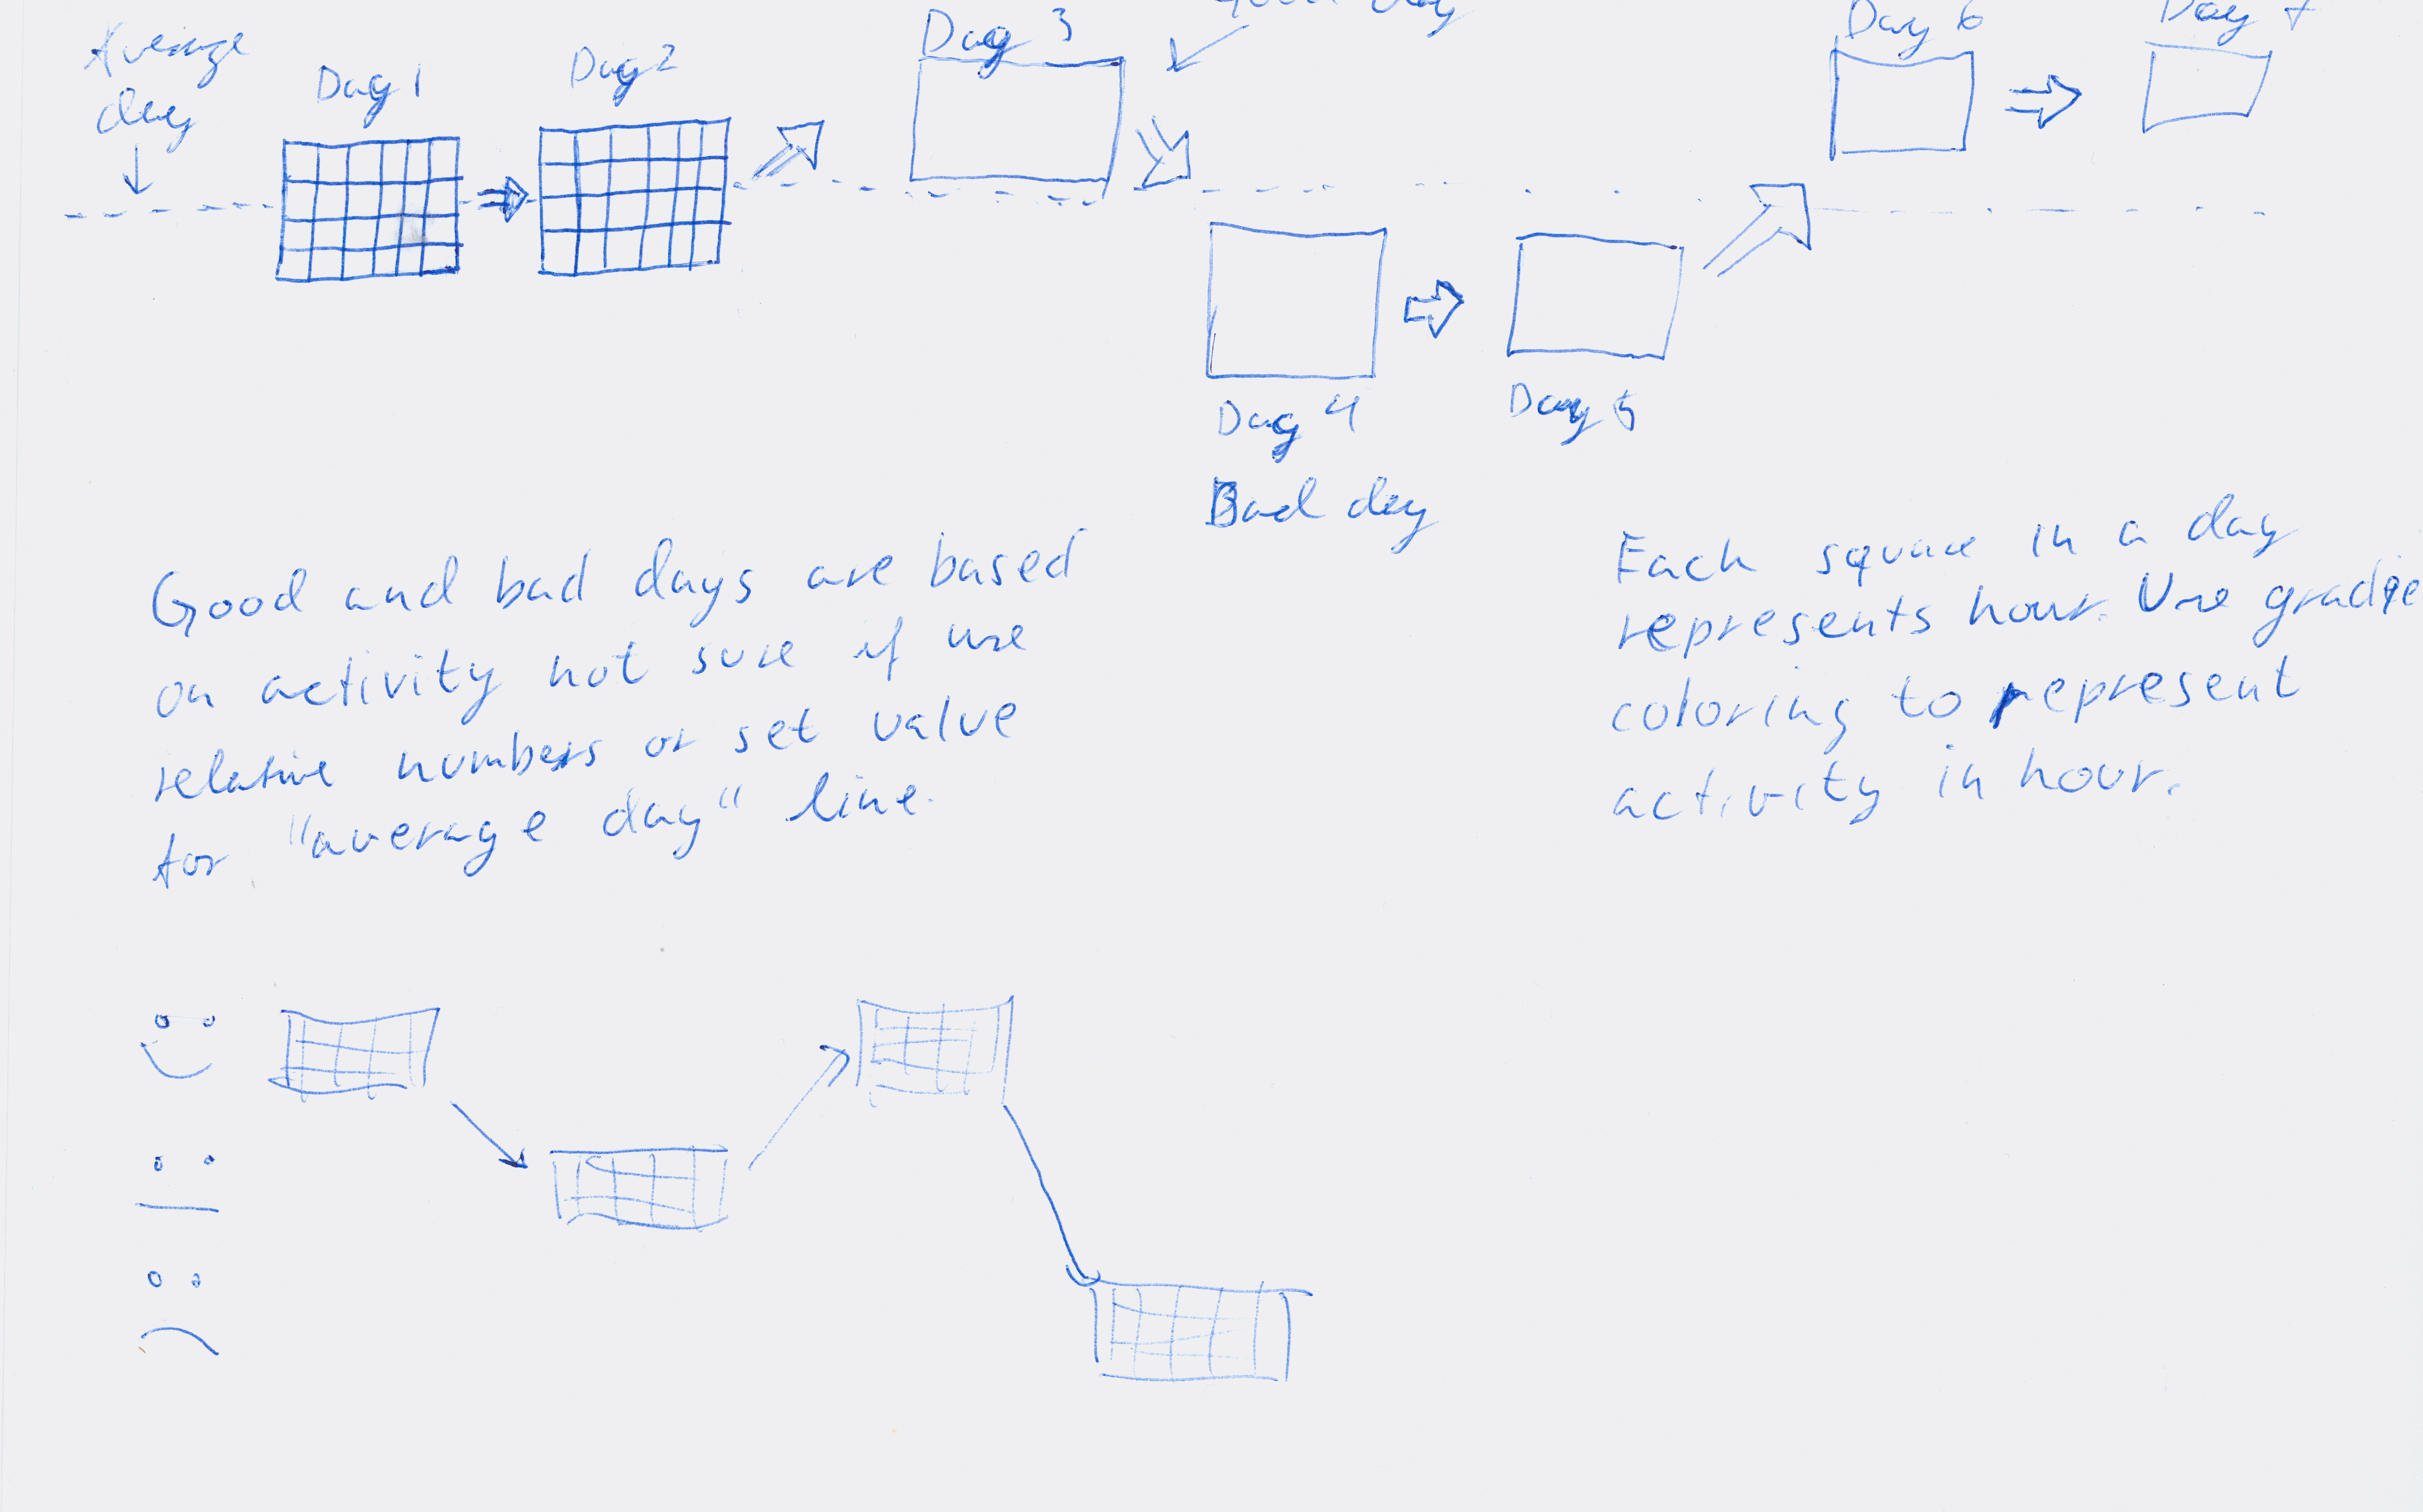
\includegraphics[width=0.6\textwidth]{detailedWeekSketch.png}
		\caption{\footnotesize Some explanation here.}
		\label{fig:detailedWeek}
\end{figure}

\section{Programming framework}
The task was to create custom visualizations form data gathered the activPAL sensor. The choice of programming tools fell on HTML5 and an open source JavaScript framework called D3.js.

\subsection{HTML5}
HTML is a markup language for the creation of web pages. HTML describes the structure and the contents of the web page. In later years, the need for advanced styling and complex interaction with web pages has made CSS and JavaScript increasingly popular. HTML5 was created as a response to this, HTML5 is an umbrella term for creating web pages using HTML5, CSS3 and JavaScript.

HTML5 has simplified the syntax compared to earlier versions. New tags have been added to better represent the modern web page elements. Other features include media tags which greatly simplifies adding multimedia content, such as playing audio and video files. More importantly for our project is the extensive support for interactive and animated graphics through the \emph{canvas-} and \emph{svg}-tag.

The new features of HTML5 and CSS3 make it much easier to create web applications for multiple platforms and screen sizes. After the smartphone and tablet revolution, creating responsive and adaptable websites has become more important. The new features included in HTML5 give large amount of flexibility with respect to the user interface and graphical visualizations.

\emph{Cascading Style Sheets} (CSS) is a language used to describe the styling of an HTML document. CSS documents describes the size, color and look of HTML elements. A new feature in CSS3, which is part of HTML5, is \emph{Media Queries}. With Media Queries it is possible to specify different styling relative to the size of the screen. This functionality is useful when creating applications that target devices with different screen sizes, such as smartphones, tablets and laptops. 

\subsection{Data-Driven Documents}
JavaScript is the main scripting language for web pages. It is a client-side scripting language that allows programmers to add functionality to otherwise static HTML-pages. While CSS3 takes care of the styling of HTML-elements, JavaScript is used to create customized behaviour. All modern browsers have JavaScript engines/interpreters that compile and run JavaScript code.

JavaScript is now an industry standard maintained by ECMA International. The standardized version of the script is named ECMAScript. Today, the names ECMAScript and JavaScript are used interchangeably, and JavaScript is often used to refer to ECMAScript. Because different browsers have different implementations of the JavaScript engine, slight variations in the way JavaScript code will run on these browsers exists.

Together with HTML5 and CSS3, JavaScript is great for creating web applications that can be designed to run on both mobile and stationary devices. JavaScript has a multitude of useful open source libraries that can be used to create complex user interaction, animation, and custom graphics.

One of the challenges in this project was to create different visualizations to represent the activity patterns of subject. Creating custom graphics in HTML5 can be done using both the canvas- and the svg-tag. In this project \gls{svg} is used. \gls{svg} is an image format that uses XML encoding to define shapes, lines, colors, and text. One benefit of this, compared to other image formats, is that details in \gls{svg}-images will not be lost when zooming. All popular browsers, and most mobile devices, support rendering of the \gls{svg}-images.

Creating graphics using svg-tags directly is cumbersome and time consuming. \gls{d3} is an open source framework that greatly simplifies this task. \gls{d3} is written in JavaScript and designed to be used in combination with HTML5. The framework can be used both to create new \gls{svg} images from scratch or modify and edit existing images. Another feature is the ability to easily add interactivity and animation to the \gls{svg}-elements. HTML5 in combination with \gls{d3} gives us flexibility to create almost any type of visualization and adding interactivity and animation to it.

%Her skriver du bare om hvordan ting ser ut, burde vi relatere det mer til sketchene, eller user requireents som jeg nevnte i paper sketches, slik at det blir en mer ``rød tråd'' over det hele. Det er kanskje ikke nødvendig her, men det burde i såfall gjøres under prototype 2. Ellers liker jeg oppstett på kapitellet, jeg har gått gjennom og endret litt tekst her og der samt gramatiske feil
\section{Running prototype}
9 of the paper prototypes were selected for implementation for the system shown to focus group 1. The diagrams were given ID, as seen in the table~\ref{tab:runProtDesc1}. Figure~\ref{fig:runProt1} shows a screen shot of the different types of diagrams. 

\begin{table}[h!]
  \begin{center}
  \begin{tabular}{|c|p{10cm}|}
    \hline
    \textbf{ID} & \textbf{Description} \\ \hline
    U1 & Classifies each day of the week into either of three categories: High, medium and low activity. \\ \hline
    U2 & Classifies each day of the week as in U1. Also shows 24 squares for each day, each square representing one hour. The activity level for each hour is displayed using a gradient. \\ \hline
    F1 & Pie chart showing the amount of activity for each day. \\ \hline
    F2 & Same as F1, but with boxes instead of pie slices and descriptive figures inside each box. \\ \hline
    F3 & Bubble chart. Divides the pie slices of F1 into bubbles each bubble representing one interval of activity (ex. 2 hours of non-stop sedentary behaviour). \\ \hline
    T1 & Timeline of 24 squares, each square represents 1 hour of activity. The amount of activity in that hour is displayed using a gradient. \\ \hline
    T2 & Rectangle shaped timeline, showing the type using colour coding. \\ \hline
    T3 & Two 12-hour clocks showing the activity type using colour coding. \\ \hline
    T4 & One 24-hour clock showing the activity type using colour coding. \\ \hline
  \end{tabular}
  \end{center}
  \caption{Diagrams implemented for the first focus group.}
  \label{tab:runProtDesc1}
\end{table}

The two diagrams U1 and U2 are week overviews. These are designed to give you a quick overview of the week. U2 experiments with adding more detail, and contains 24 small squares for each day that represent the activity of each hour. Holding the mouse cursor over a day in U1 will show the percentage of each type of activity for that day. Holding the mouse cursor over a square in U2 will show the percentage of each type of activity for the hour that square represents.

\begin{figure}[h!]
  \centering
  \begin{subfigure}[b]{0.45\textwidth}
    \centering
    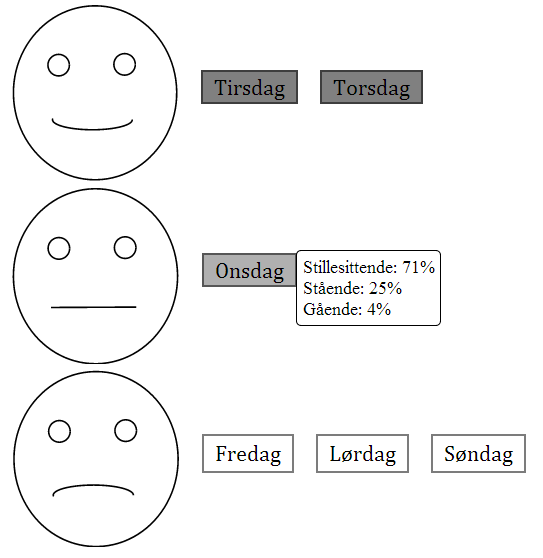
\includegraphics[width=\textwidth]{u1First.png}
    \caption{U1}
  \end{subfigure}
  \begin{subfigure}[b]{0.45\textwidth}
    \centering
    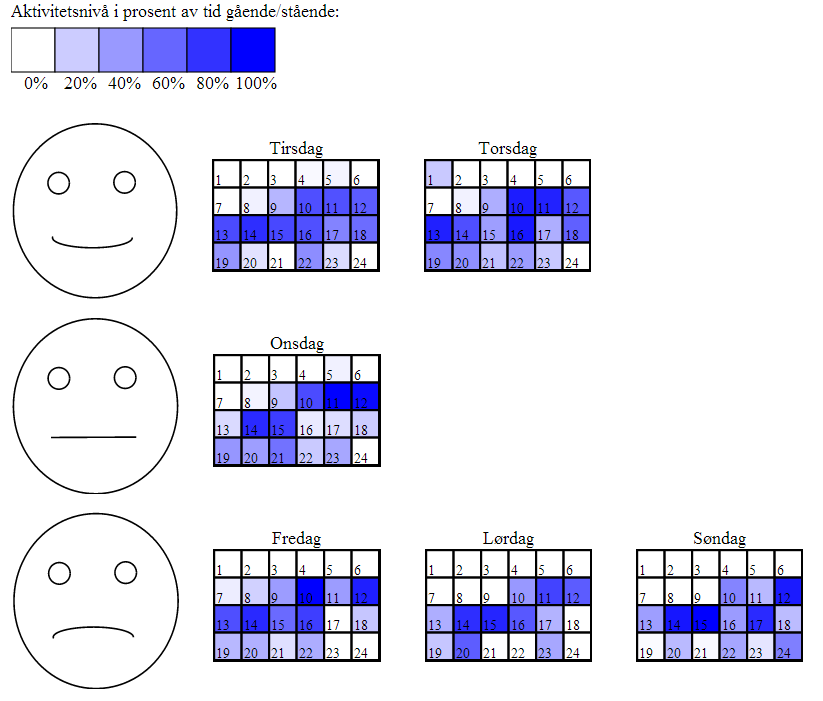
\includegraphics[width=\textwidth]{u2First.png}
    \caption{U2}
  \end{subfigure}
  \caption{Week overview charts.}
  \label{fig:runProt1}
\end{figure}

%Review: Tror du har mistet now tekst det står bare ``When showing the entire week'' og så slutter det.
Diagrams F1, F2 and F3 are the fractional charts*. These diagrams shows the fraction of each type of activity for a day. F1 and F2 are similar, F1 is a standard pie diagram while F2 uses boxes with figures describing the activity. F1 and F2 has two types of view modes: one day or the entire week. When showing the entire week. F3 is more complex, this diagram shows each interval of activity as a ball. Long intervals of activity is represented by a larger ball than small intervals of activity. This graph can therefore be used both to see the distribution of the different activity types and, more importantly, the length of continuous activity, or sedentary behaviour. This is useful when you want to identify if the patient has very long periods of sedentary behaviour, or if the patient walks continuously for a long time, or takes small brakes. Holding the mouse cursor over a bubble shows you the time the activity interval occurred as well as the length of the interval. F3 also offers a highlighting mode, when active intervals of more than 1 hour are highlighted.

\begin{figure}[h!]
  \centering
  \begin{subfigure}[b]{0.45\textwidth}
    \centering
    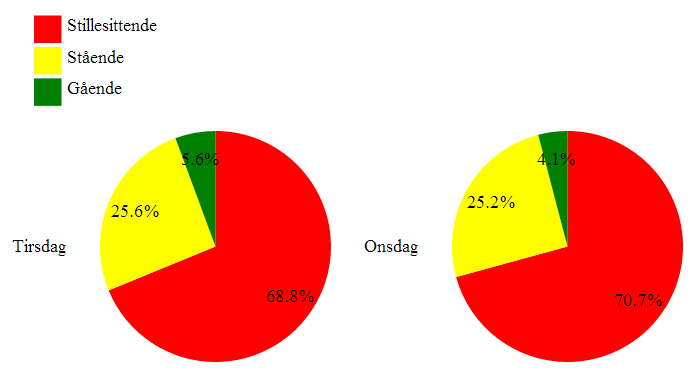
\includegraphics[width=\textwidth]{f1First.png}
    \caption{F1}
  \end{subfigure}
  \begin{subfigure}[b]{0.45\textwidth}
    \centering
    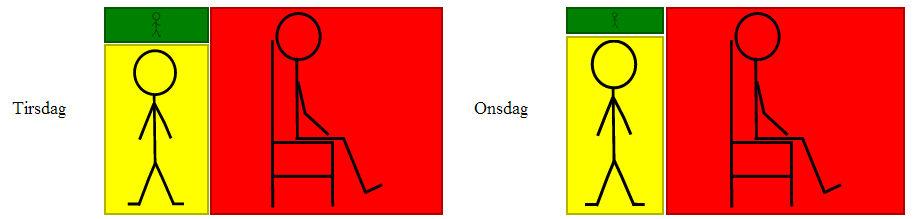
\includegraphics[width=\textwidth]{f2First.png}
    \caption{F2}
  \end{subfigure}
  \\
  \begin{subfigure}[b]{0.45\textwidth}
    \centering
    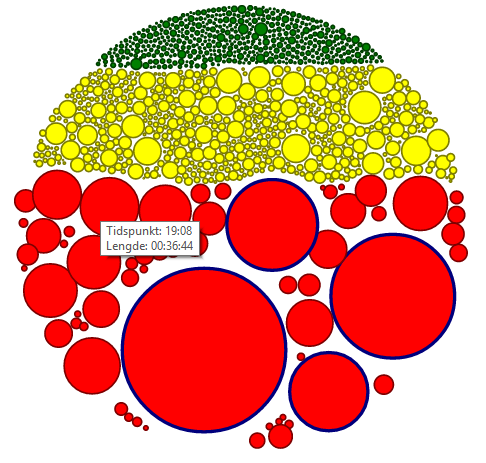
\includegraphics[width=\textwidth]{f3First.png}
    \caption{F3}
  \end{subfigure}
  \caption{Fractional charts*}
\end{figure}

T1, T2, T3 and T4 are diagrams that show timelines or clocks. These diagrams are useful to see when the patient was active during the day. T1 shows 24 squares each representing an hour of the day. The percentage of activity (walking and standing) is shown as a gradient in each square. Holding the cursor over a square gives you the percentage of each type of activity. T2 is also a timeline, but here the data is not aggregated so the timeline is continuous and shows the activity at a much more detailed level. This is useful if you need to see when in a particular hour activity was performed. It also distinguishes between standing and walking activity. T3 and T4 are also show the activity continuously but they use a clock instead of a timeline to illustrate when on they day the activity occurred. T3 uses two 12 hour clocks, while T4 uses a single 24-hour clock. Diagrams T2, T3 and T4 can toggle highlighting. When highlighting is toggled sedentary behaviour longer than 1 hour is highlighted with blue. All T-diagrams can be viewed one day at a time or the entire week all at once. 

\begin{figure}[!h]
  \centering
  \begin{subfigure}[b]{0.45\textwidth}
    \centering
    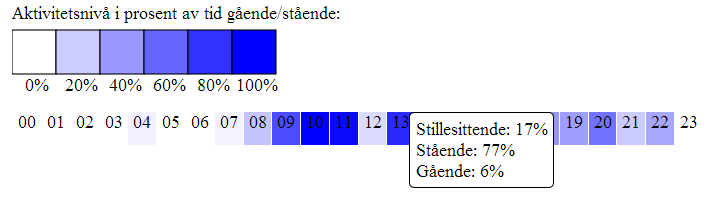
\includegraphics[width=\textwidth]{t1FirstSingle.png}
    \caption{T1 day.}
  \end{subfigure}
  \begin{subfigure}[b]{0.45\textwidth}
    \centering
    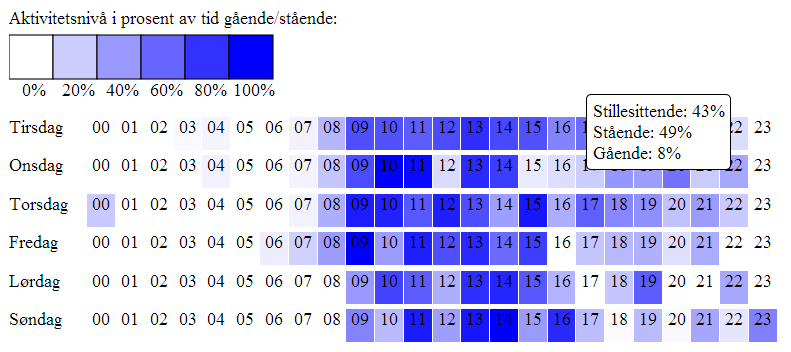
\includegraphics[width=\textwidth]{t1FirstWeek.png}
    \caption{T1 week.}
  \end{subfigure}
  \\
  \begin{subfigure}[b]{0.45\textwidth}
    \centering
    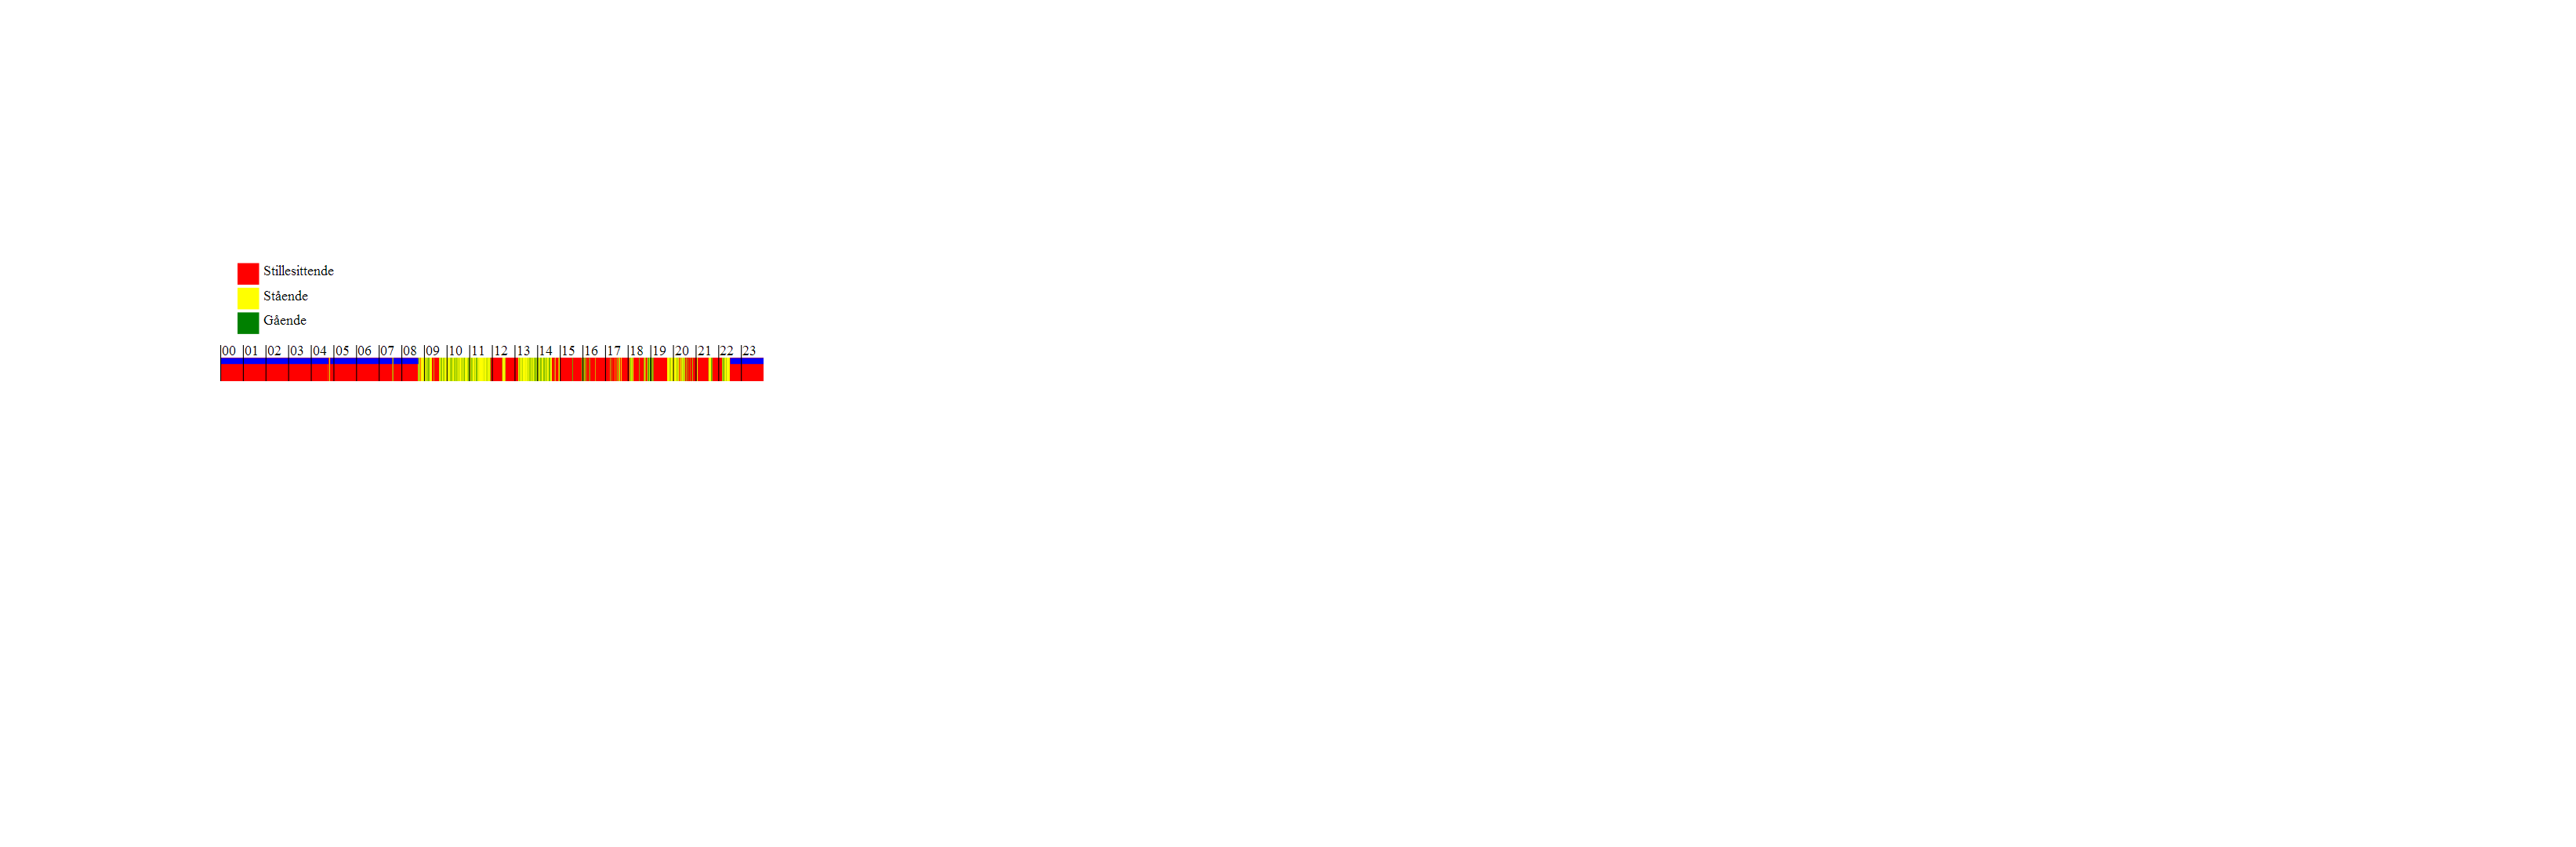
\includegraphics[width=\textwidth]{t2FirstSingle.png}
    \caption{T2 day.}
  \end{subfigure}
  \begin{subfigure}[b]{0.45\textwidth}
    \centering
    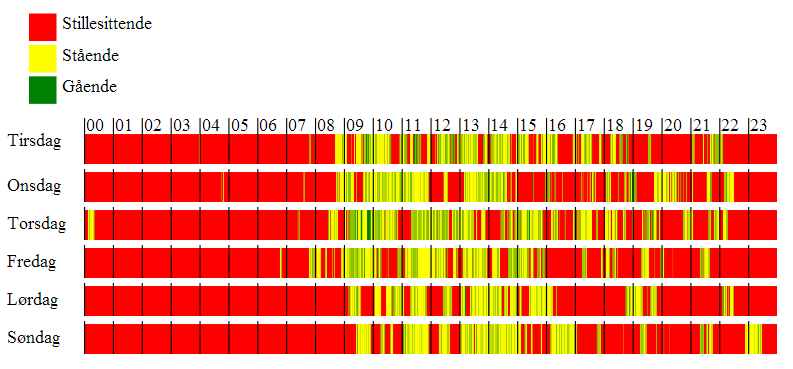
\includegraphics[width=\textwidth]{t2FirstWeek.png}
    \caption{T2 week.}
  \end{subfigure}
  \\
  \begin{subfigure}[b]{0.45\textwidth}
    \centering
    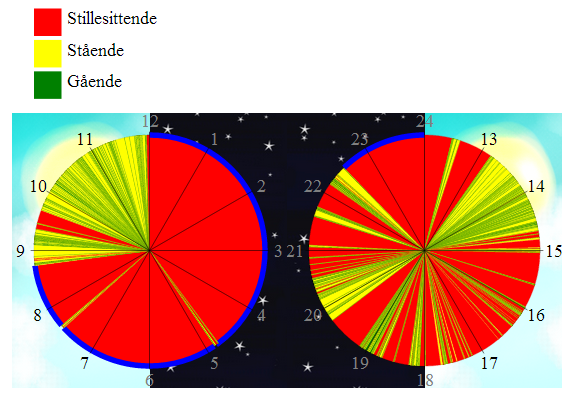
\includegraphics[width=\textwidth]{t3First.png}
    \caption{T3}
  \end{subfigure}
  \begin{subfigure}[b]{0.45\textwidth}
    \centering
    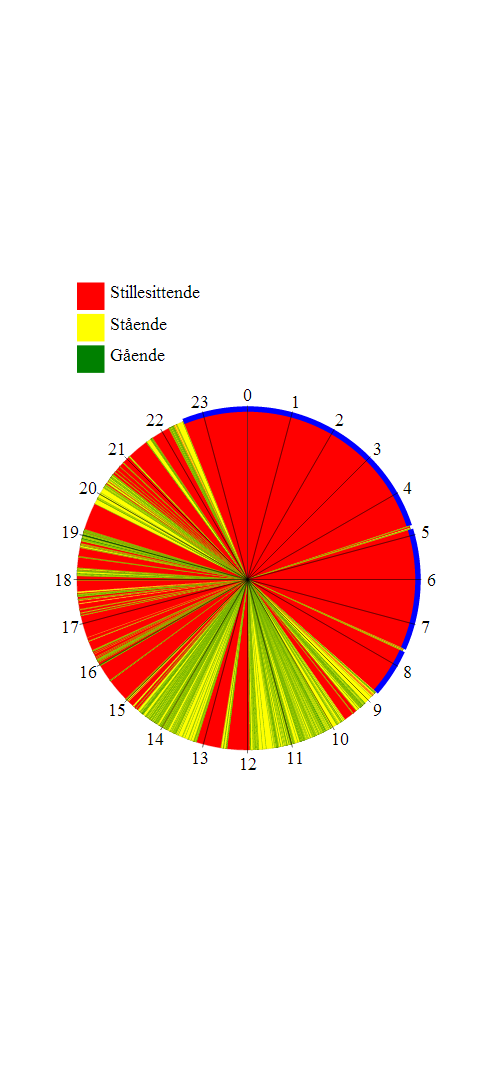
\includegraphics[width=\textwidth]{t4First.png}
    \caption{T4}
  \end{subfigure}
\end{figure}  
